\documentclass[11pt]{article}


\setlength{\oddsidemargin}{-0.25 in}
\setlength{\evensidemargin}{-0.25 in}
\setlength{\topmargin}{-0.9 in}
\setlength{\textwidth}{7.0 in}
\setlength{\textheight}{9.0 in}
\setlength{\headsep}{0.75 in}
\setlength{\parindent}{0.3 in}
\setlength{\parskip}{0.1 in}
\usepackage{epsf}
\usepackage{pseudocode}
\usepackage{dsfont}
\usepackage{amssymb}
\usepackage{amsmath}
\usepackage{graphicx}
\usepackage{mathtools}
\DeclarePairedDelimiter\ceil{\lceil}{\rceil}
\DeclarePairedDelimiter\floor{\lfloor}{\rfloor}

\renewcommand*\contentsname{Summary}



\begin{document}
\title{Programming Assignment 3\\
CS 124}
\author{Artidoro Pagnoni, Nisha Swarup}
\date{\today}
\maketitle

\tableofcontents
\clearpage
\section{Dynamic Programming Solution to Number Partition Problem}
\subsection{General Idea}
Although the Number Partition Problem is NP complete, we can solve it in pseudo-polynomial time. Let $b$ be the sum of all $n$ integer entries of $A$. The solution that we will propose is polynomial in $nb$. In the Number Partition Problem we are essentially creating two sets with the least possible difference. 

Our solution lies on the computation of all possible partitions of the initial subset of elements into two sets. We only care about the possible values that can be reached by the sum of the elements in every partition. Since the sum of all entries of $A$ is $b$, we are interested in knowing all the possible values in the range $[0,b]$ that can be reached by creating a subset of the first elements of $A$ and summing over all elements of the subset. We can imagine this information is stored in an array of length $b$, in which a 1 in position $j$ means that $j$ is the result of the sum of the elements of the first $i$ elements of $A$. If $j$ is not the sum of the elements of a subset, then the jth entry in the array will be 0.  Given such an array we can find the value that is closest to $b/2$. The closer we get to $b/2$, clearly the lower the residue between the two subsets will be. 

\subsection{Recurrence}
We can calculate this solution recursively. The recursion is done on the initial set. At every step we include one more element in the initial set, eventually covering the whole set. Given the solution array at one step, we can calculate the solution array at the next step in the following way. All the values that could be reached at the previous step can still be reached (we can choose the same subsets, and just discard the new element). In addition, we can choose subsets that include the new element. This will increase the value of the sum of their elements by the the new element. 

We can formalize this by filling out a matrix $M$ of size $n\times b$, such that the rows correspond to the solution arrays mentioned above. The first row is the base case, and corresponds to the empty set (when we don't include any element of $A$). As we increase the row number, we add more elements of $A$ to the initial set. The columns correspond to the values of the sum that need to be reached.
We therefore have:

Recurrence Relation:
\begin{eqnarray}
M_{(0,0)} &=& 1\\
M_{(0,j)} &=& 0 \;\;\;\;\;\;\;\;\;\text{for $j \neq 0$}\\
M_{(i,j)}&=&\max\{M_{(i-1,j)},M_{(i-1,j-A_i)}\}
\end{eqnarray}

$M_{(i,j)}$ is 1 if we can reach $j$ with the sum of the first $i$ elements of $A$. The base case is clear, with no elements we can only reach value 0.

The recurrence equation is also quite straightforward. The first term is 1 when you could reach $j$ at the previous step, (without the new element). The second term is 1 when we can reach $j$ by adding $A_i$ (the new element) to any of the values at the previous step. The max ensures that if any of the two terms is 1, we will get 1 out (it serves the same purpose as an or, if we use booleans instead of 0s and 1s).

We fill out the matrix row by row from left to right, following the recurrence equation.

Once we have the matrix, we will only consider the last row, and find the closest reachable value to $b/2$. We can therefore run through the last row starting at $\floor*{b/2}$ and finding the first non zero entry. One subset will have the value corresponding to the index of the column of the first non zero entry, and the other will have the complement of that index ($b-j$).

The residue can be calculated by taking the absolute value of the difference of the values found for the two subsets.

\subsection{Reconstruction of the Subsets}
This algorithm finds the minimum residue but does not tell us how to partition the set $A$. If we want to construct the two subsets, we need to fill out an addition matrix, of the same size. The matrix will be composed of pointers to the parent entry. By parent we mean the entry that was equal to 1 in the equation $M_{(i,j)}=\max\{M_{(i-1,j)},M_{(i-1,j-A_i)}\}$. If both terms were 1, pick the first.

To reconstruct the subset we need to find for every element if they belong to one set or the other. We will start with the last element in $A$. We take the last row in the Pointer's matrix, and the column that corresponds to one of the subsets,(the closest possible to $b/2$). If the pointer is pointing to the same column then the element in consideration is in set 1, if not it is in set 2. The next element to be considered is the one pointed to by the pointer, and we repeat the same reasoning until we get to the first element.

\subsection{Further Optimization}
We notice that we don't really need to complete the right half of either matrices. It is a question of symmetry - if one set has a total sum below $b/2$, the other will be above. Therefore, we need to make sure to fill out the matrix up to column $\ceil*{b/2}$. We will start at $b/2$ and go down in the last row when looking for the closest reachable entry to $b/2$.
This saves half of the time and space, but will not change the asymptotic running time. 

\subsection{Space and Time Complexity}

In terms of space complexity, this algorithm is $O(nb)$, since we need to fill out two matrices of size $n\times b/2$.

The time complexity is polynomial in $nb$ more precisely it is $O(nb)$ since we need to fill out the entire matrix and every entry requires a constant number of operations (two comparisons and writing to both the solution and the pointer matrix). This confirms that we have a pseudo-polynomial solution for the Number Partition Problem. 




\section{Karma Karp Algorithm Time Complexity}
The Karma Karp algorithm can be implemented in $O(n\log n)$. 
We will describe the algorithm that we have implemented.

We construct a binary Max Heap with the initial set. Inserting something in the Max Heap takes at most $O(\log n)$, and we are doing it for every element in the set. Therefore the total time from the construction of the Max Heap is $O(n \log n)$.

Once we have the Max Heap constructed, we need to extract the two largest elements. This corresponds to two Delete Min operations, which take $O(\log n)$ each. We then take the difference of the two elements and insert it back to the Max Heap, also with time $O(\log n)$.

We repeat the last step exactly $n-1$ times. At every step we reduce the size of the Max Heap by 1 (two delete min and one insert). We have an initial size of $n$ and we need to get down to $1$, which takes $n-1$ steps.

Now putting everything together we have a run time of:

\begin{eqnarray}
&&\text{Construct Max Heap} + (n-1)(\text{2 Delete Min}+\text{Insert})\\
&=& O(n \log n)+(n-1)(2*O(\log n)+O(\log n)))\\
&=& O(n\log n) + O(n\log n)\\
&=& \boxed{O(n\log n)}
\end{eqnarray}

This shows that our algorithm implements Karma Karp in $O(n\log n)$.

\section{General Discussion of our Implementation}
\subsection{Description of Algorithms}

We used Python to complete this assignment.

Our KK algorithm relies on a binary Max Heap.


For each representation we had 3 functions: calculate-residue, generate-random-soln, and random-move, which are self-explanatory. 

Random move returns an array of swaps to make on the random move. We then passed these functions in as parameters to the functions for each of the three algorithms that we wanted to implement. For the simulated annealing function, we used the suggested cooling schedule. This affects the probability of keeping a worst solution.



\subsection{Complications}

One complication we faced was that Python is neither a call-by-value nor a call-by-reference language, but a mixture of the two since it is call-by-object. We spent a while debugging one method since the immutable / mutable object dichotomy is a very different framework than that of Java or C++. This was a very valuable learning experience in how to maintain objects to write good Pythonic code.


\section{Results and Analysis}
\subsection{Relative Performances}
We see that representation two takes significantly more time to run, but also has significantly better performance among all three of the algorithms. KK is very fast because we are only running it once. It makes sense that repeated random takes slightly longer than the other two algorithms since we are generating more random numbers, which makes a difference over 25,000 trials. It makes sense that representation 2 takes more time than representation 1, since representation 1 just adds numbers to calculate residues which takes linear time, whereas representation 2 has to run KK which will take $O(n\log n)$ every time. 

\begin{center}
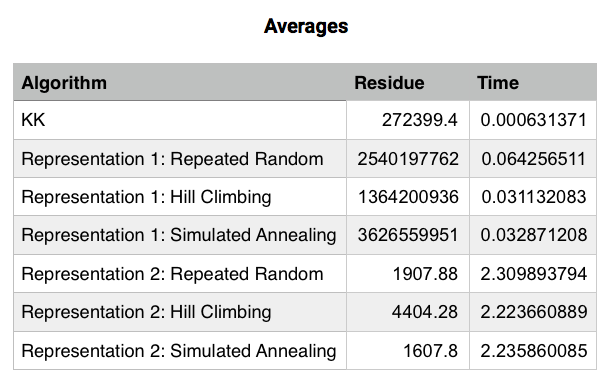
\includegraphics[scale=0.9]{avtab.png}
\end{center}

\subsection{Differences in Solution Space}

\begin{center}
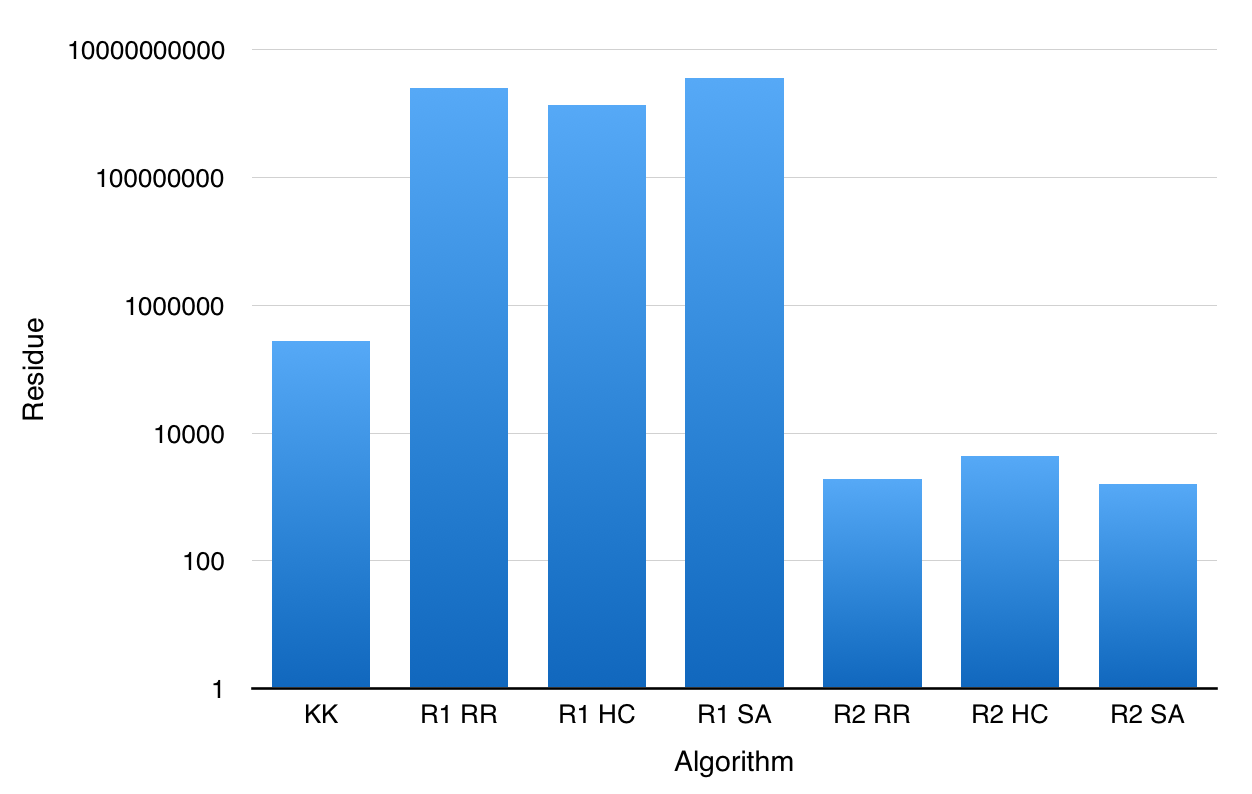
\includegraphics[scale=0.5]{avinsto.png}
\end{center}
The above graph shows the average residues for each algorithm on a logarithmic scale. 

We see that KK performs better than the first representation, but worse than the second representation. This shows us that a random algorithm’s performance is heavily affected by the representation of solutions or in other words, how we set up the problem. This matters more than the actual algorithmic method that we use. 

In the standard representation a neighbor's residue will vary significantly from its ancestor. On average, a change consists in swapping one element from one side to the other, and since we are considering extremely large elements (order of $10^12$) we have very large differences. Even when we are swapping two elements, the expected difference in residue is still of almost the same order of magnitude as the elements (one less). This makes it harder to find a local improvement. We can understand this as the solution space being more bumpy when using the standard representation.

By setting up the problem with representation 2, we change how we choose moves between solutions and hence change how many local optima there are. In this case, the difference in residue between two neighbors can be smaller. It may seem counter-intuitive since prepartition will create individual elements that are very large. However, their size will be compensated within the algorithm by putting more larger elements on the other side. This creates a smoother solution space. 

This means that the solution space for representation 1 would be more bumpy, whereas the solution space for representation 2 would have less bumps.

\subsection{Karma Kart Residue Frequency Plots}
\begin{center}
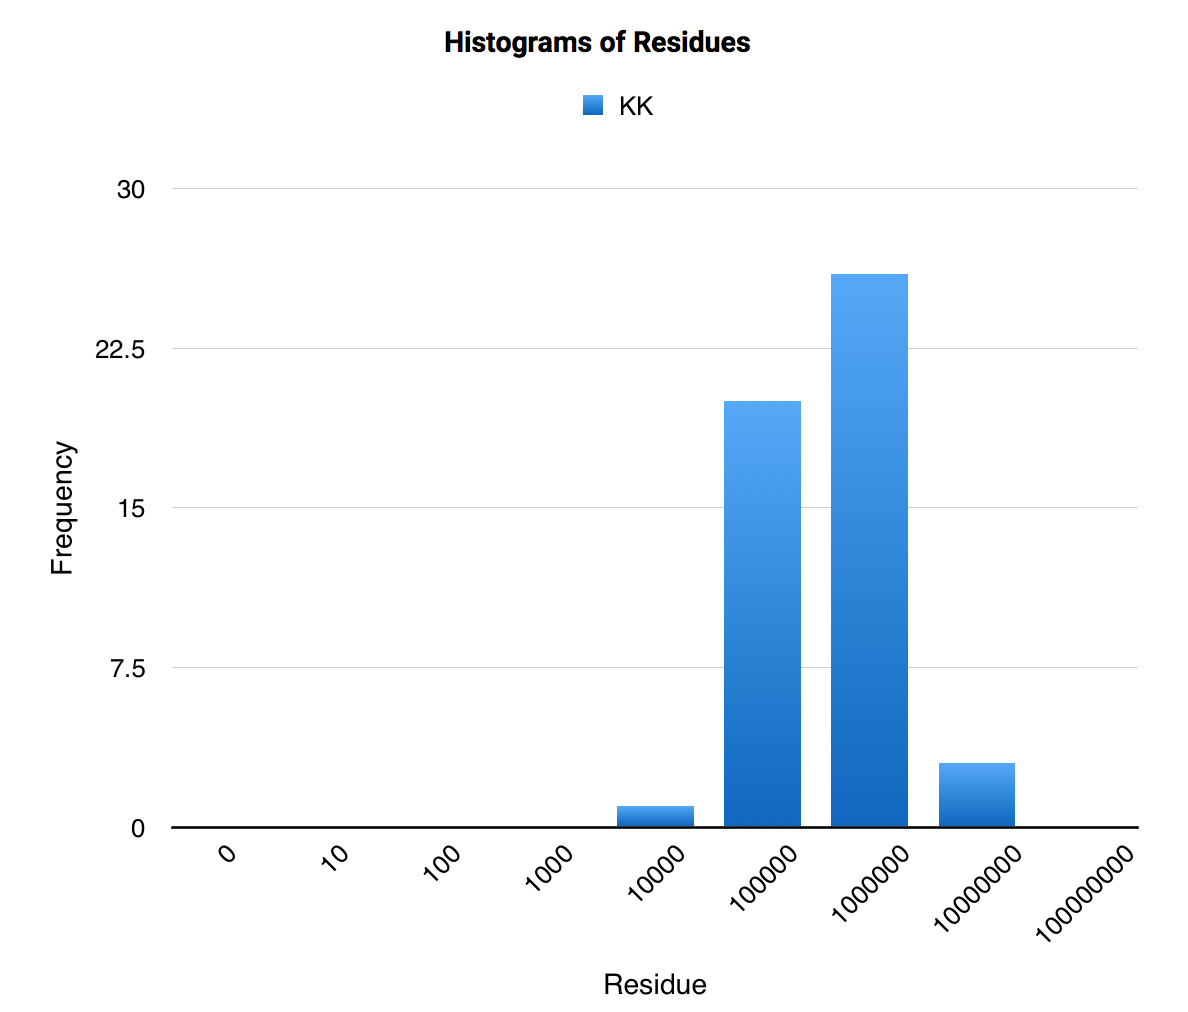
\includegraphics[scale=0.5]{kkinsto.png}
\end{center}


Here is a histogram of residues for the Karmarker-Karp algorithm. We see that the algorithm mainly produces residues less than 100,000, although there will be outliers on the right. Residues of 100,000 are pretty good for random integers on the interval [0 to 1,000,000,000,000].



\subsection{Frequency Tables in the Appendix}
In the Appendix  you will find frequency tables of residues for each of the algorithms and each of the representations. We used raw number frequencies instead of proportions, since there was an equal number of trials for each algorithm (50 instances). In the legends for the graphs, R1 means representation 1, R2 means representation 2, RR means repeated random, HC means hill climbing, and SA means simulated annealing. 



\subsection{Residue Plots}
The graphs in the Appendix show how the residue changes by iteration on a new generated instance. We show the iteration on the x-axis and the residue on the y-axis. The residue is close to its final value after the 15,000th iteration, and this is because the solution space gets flatter as we get closer to optimal value. This is a characteristic of constraint optimization problems. 
 
We also see that the residue for the second representation RR in this particular instance that we generated was under 100. This goes to show how much results vary by the instances that are generated, due to randomness. 

Finally, we also notice that for the Standard Representation the improvements in the residue values are always very large. In the Prepartition representation the improvements are large at first   but get to less than 1000. The smaller improvements allow for a lower overall residue. This confirms that the solution space in the Prepartition Representation is smoother and allows for small improvements. 

\subsection{Distribution of Repeated Random Results}
The Repeated Random algorithm has similar looking distributions across both representations. This makes sense because it just generates a bunch of random options and chooses the optimal one.



\section{Karma Karp as Starting Point for the Randomized Algorithms}
The implementation of Karma Karp that we have provided returns a residue but does not construct the corresponding partition. We could easily construct it with a slight variation, as suggested in the prompt.

Supposing that we get the partition from the Karma Karp algorithm, we can use that partition as a starting point instead of generating a random one.

The first thing to notice is that the three algorithms always return the best solution found. Using the Karma Karp partition as a starting point ensures that we will never get a worse solution. Starting with Karma Karp will have different effects for the two representations.

\textbf{Standard vs Prepartition:}
In the Standard Representation starting with Karma Karp would start our optimization from that point in solution space. We therefore expect our solution to slightly improve from the Karma Karp solution, but only slightly. It would only slightly improve because it would quickly get stuck in local minima. Here, the solution space is not very well defined. 

With the Prepartition representation, the optimization from the Karma Karp solution would still reduce the residue significantly. We expect the solution to be lower than the solutions obtained without starting with Karma Karp. Here it is harder to get stuck in local minima because the solution space is defined better. 



\textbf{Repeated Random:}
Starting Repeated Random with Karma Karp has the effect of only adding to the randomly generated solution the Karma Karp solution. As we have seen in the previous graphs, Karma Karp usually offers a significantly better solution than the Repeated Random Algorithm for the standard representation. Therefore, on average, we will get the Karma Karp solution back when using the variation of Repeated Random with the standard representation.

With the prepartition representation instead, Repeated Random usually generates better results than Karma Karp. So adding the Karma Kart solution to the solution set won't affect the result of the algorithm.



\textbf{Hill Climbing:}
When we start Hill Climbing with Karma Karp we are actually starting with an already fairly optimized solution. What will happen is that improvements will be less frequent. This means that the curve of residue in time will be flatter. As we get closer to the optimized value the solution space gets flatter and flatter. 


%The risk is to hit a local minimum with the Karma Karp solution. The Hill Climbing approach may miss to get out of the local minimum since it moves to a neighboring solution only if it is better than the current one. This is particularly relevant to the standard representation, which as it appears from the graphs presented above tends to get stuck to local minima very quickly.  If the Karma Karp solution is a local minimum, and the Repeated Random can't get out of it, it will just return that as solution.  
%
%The prepartion representation will likely improve on the Karma Karp solution. 



\textbf{Simulated Annealing:}
Similarly, starting with the Karma Karp solution corresponds to starting with an already fairly optimized solution. Here as well, the frequency of the improvements will be lower. This means that the curve of residue in time will be flatter. 


\clearpage















\end{document}